\problemname{The Expression}

Hedvig has been given the homework of evaluating a long arithmetic expression. It consists of non-negative integers separated by the operators +, - and * (plus, minus and times). However, she does not need to use the usual precedence rules; instead she can freely choose two adjacent numbers with an operator between them, evaluate this expression, and replace the expression with the result of the operation. The procedure is repeated until only one number remains: the result of evaluating the entire expression.

Write a program that computes the largest possible result Hedvig can get.

\begin{figure}[ht!]
\centering
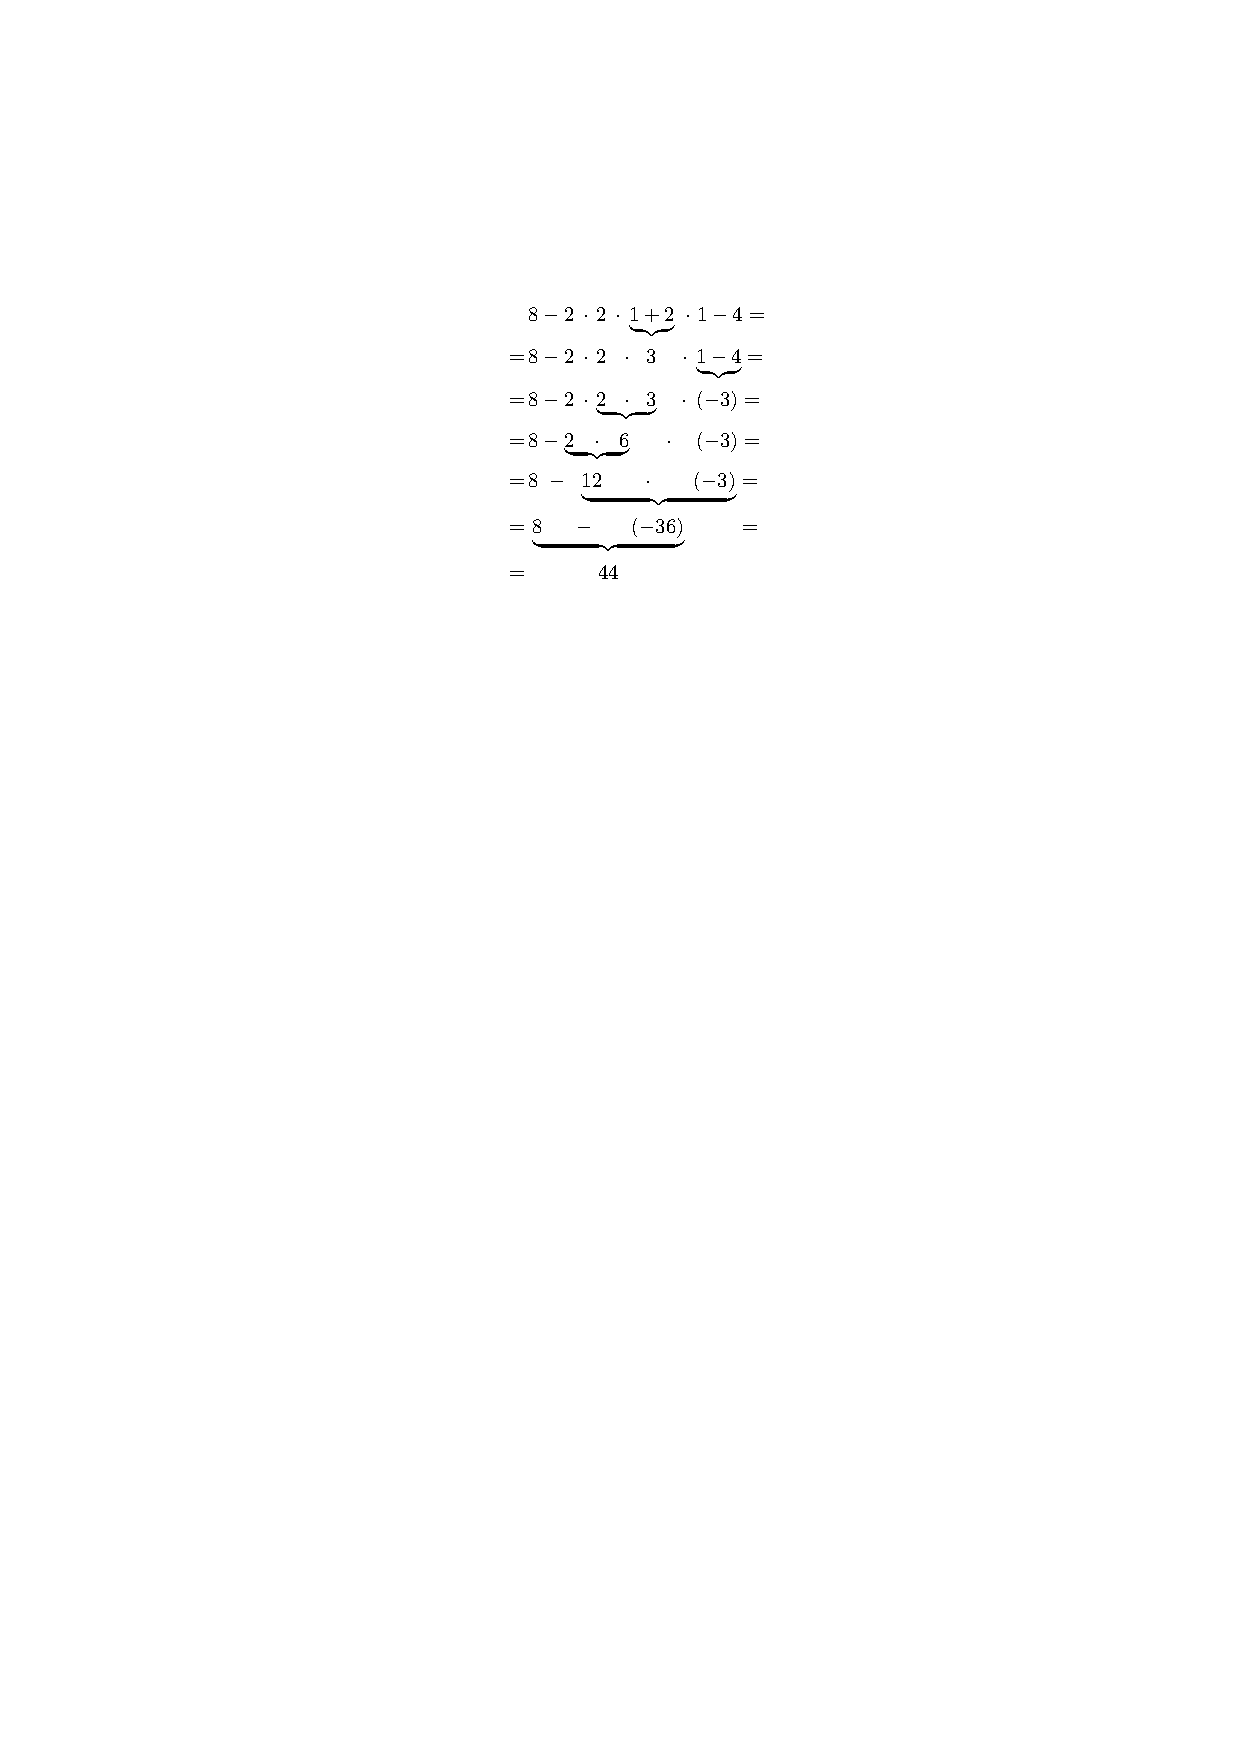
\includegraphics[width=0.4\textwidth]{example.pdf}
\caption{An optimal evaluation order in the second example.}
\label{overflow}
\end{figure}

\section*{Input}

The first line contains a string of at most 100 characters: the expression to be evaluated. It follows the pattern \newline
[number] [operator] [number] [operator]....[operator] [number] \newline
without any spaces. Each operator is either +, - or *, and each number $k_i$ satisfies $0\leq k_i < 1{,}000{,}000$. No number is written with superfluous leading zeros.

\section*{Output}

An integer: the largest value that can be obtained by evaluating the expression in any order. This number, as well as all possible intermediate results that can occur, is always greater than $-10^{18}$ and less than $10^{18}$.


\section*{Scoring}
Your solution will be tested on several test groups. To earn points for a group,
you must pass all test cases in that group.

\begin{tabular}{| l | l | l |}
\hline
Group & Points & Constraints \\ \hline
1     & 11         & Only the operators + and * appear. The number of terms is at most 10 and they satisfy $1\leq k_i \leq 9$. \\
2     & 11         & All operators may appear. The number of terms is at most 10. \\
3     & 37         & Only the operators + and * appear.\\ 
4     & 41         & All operators may appear. \\ \hline
\end{tabular}
